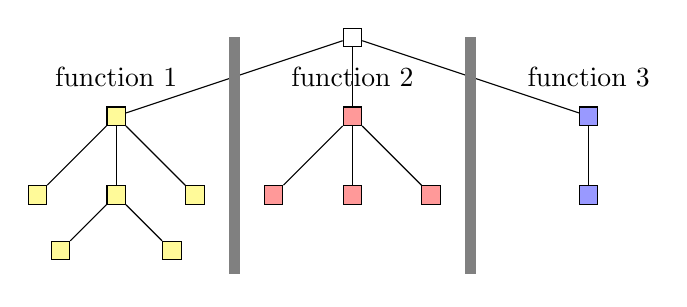
\begin{tikzpicture}[
>=stealth,
line/.style={draw},
bigl/.style={draw,line width = 4pt, color=black!50},
root/.style={draw},
func1/.style={draw,fill=yellow!40},
func2/.style={draw,fill=red!40},
func3/.style={draw,fill=blue!40}
]

\node[root] (root) at (0,0) {};

\node[func1] (fu1) at (-3,-1) {};
	\node[func1] (fu12) [below of = fu1] {};
	\node[func1] (fu13) [right of = fu12] {};
		\node[func1] (fu131) [below right of = fu12] {};
		\node[func1] (fu132) [below left of = fu12] {};
	\node[func1] (fu14) [left of = fu12] {};

\node[func2] (fu2) at (0,-1) {};
	\node[func2] (fu22) [below of = fu2] {};
	\node[func2] (fu23) [right of = fu22] {};
	\node[func2] (fu24) [left of = fu22] {};

\node[func3] (fu3) at (3,-1) {};
	\node[func3] (fu31) [below of = fu3] {};

\path[line] (root) -- (fu1);
	\path[line] (fu1) -- (fu13);
	\path[line] (fu1) -- (fu12);
		\path[line] (fu12) -- (fu131);
		\path[line] (fu12) -- (fu132);
	\path[line] (fu1) -- (fu14);

\path[line] (root) -- (fu2);
	\path[line] (fu2) -- (fu22);
	\path[line] (fu2) -- (fu23);
	\path[line] (fu2) -- (fu24);

\path[line] (root) -- (fu3);
	\path[line] (fu3) -- (fu31);

%separators
\path[bigl] (-1.5,0) -- (-1.5,-3);
\path[bigl] (1.5,0) -- (1.5,-3);
%functions
\node (fun1) at (-3,-.5) {function 1};
\node (fun2) at (0,-.5) {function 2};
\node (fun3) at (3,-.5) {function 3};


\end{tikzpicture}